
\chapter{Exercise 11}
\label{cha:ugeopgave-11}

The purpose of the exercise is to understand the theory behind parametric curves and surfaces and how to use this theory to create geometric models. The theory includes Bezier, uniform B-spline, non-uniform B-spline and NURBS (non-uniform rational B-spline) curves and surfaces.
The advantage of using a parametric representation of curves and surfaces is that they can be represented using only a few control points instead of a detailed mesh.


\section{Part 1}


After following descriptions given in exercise description document, I manage to implement cubic Bezier curve.

You can see a screenshot of a cubic Bezier curve in Figure \ref{fig:11-1}.




\begin{figure}[hp]
\centering
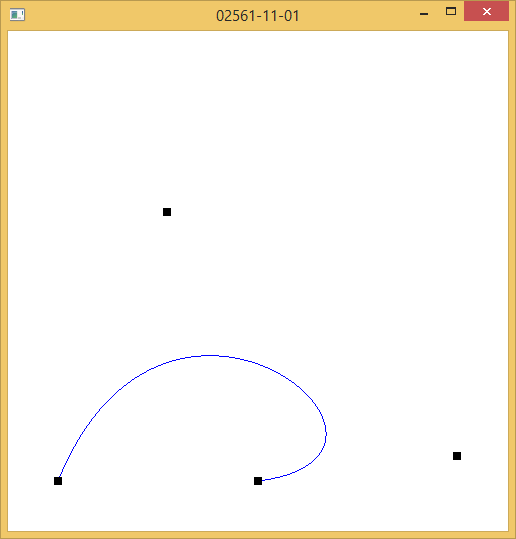
\includegraphics[width=8cm]{../Screenshots/ex-11/1.png}
\caption{A cubic Bezier curve}
\label{fig:11-1}
\end{figure}

\section{Part 2}

I carry out the part by following the description given in the text and using the knot vector given. 
A screen capture of the circle can be seen in Figure \ref{fig:11-2}.

\begin{figure}[hp]
\centering
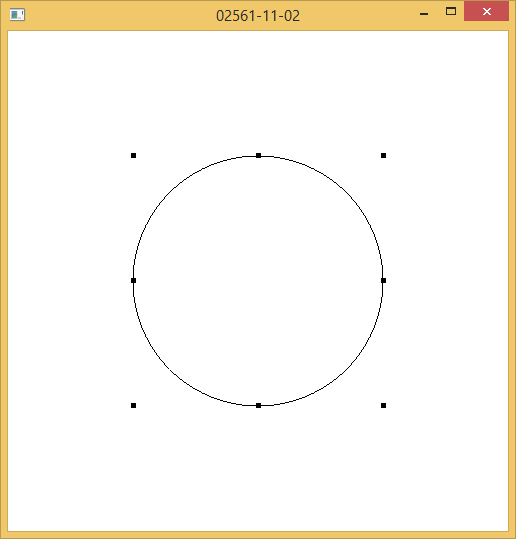
\includegraphics[width=8cm]{../Screenshots/ex-11/2.png}
\caption{The exact circle created by Bezier curves and by using NURBS}
\label{fig:11-2}
\end{figure}

\section{Part 3}



\subsection{Item 1}

Linear interpolation is already implemented. It is based on simple line segment drawing. A screenshot of these line segments can be seen in Figure \ref{fig:11-3-1}.

\begin{figure}[hp]
\centering
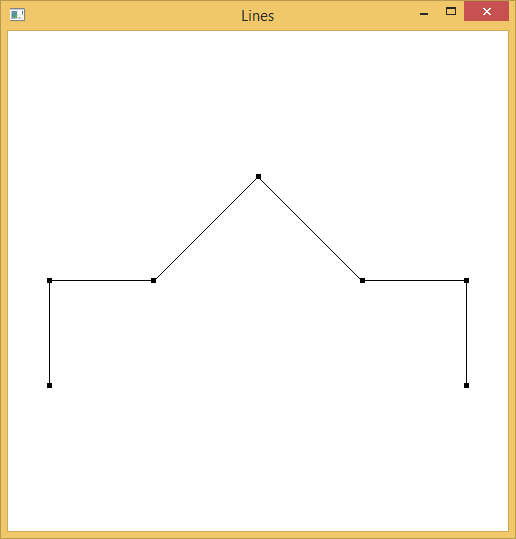
\includegraphics[width=8cm]{../Screenshots/ex-11/3-1.png}
\caption{Linear}
\label{fig:11-3-1}
\end{figure}

\subsection{Item 2}

I draw a Bezier curve in order 4 by using first 4 control points. The knot vector that is used in this item is

$ \{ 0, 0, 0, 0, 1, 1, 1, 1\} $ \\

A screenshot of these line segments can be seen in Figure \ref{fig:11-3-2}.


\begin{figure}[hp]
\centering
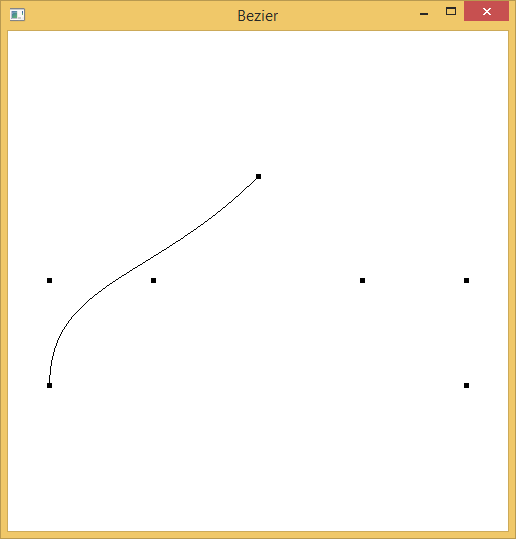
\includegraphics[width=8cm]{../Screenshots/ex-11/3-2.png}
\caption{Bezier}
\label{fig:11-3-2}
\end{figure}

\subsection{Item 3}

I draw a uniform B-Spline in degree 3 by using all control points. The knot vector that is used in this item is\\

$ \{0, 1, 2, 3, 4, 5, 6, 7, 8, 9, 10\} $ \\

\noindent
A screenshot of the curve can be seen in Figure \ref{fig:11-3-3}.


\begin{figure}[hp]
\centering
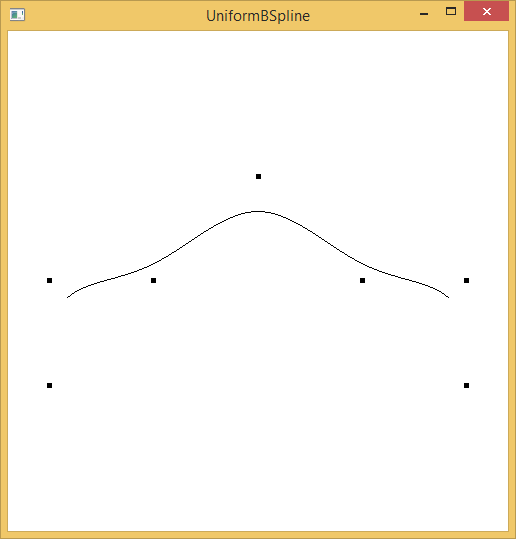
\includegraphics[width=8cm]{../Screenshots/ex-11/3-3.png}
\caption{Uniform B-Spline}
\label{fig:11-3-3}
\end{figure}

\subsection{Item 4}

I draw a nonuniform B-Spline in degree 3 by using all control points. The knot vector that is used in this item is\\

$ \{0, 0, 0, 0, 1, 2, 3, 4, 4, 4, 4\} $ \\

\noindent
A screenshot of the curve can be seen in Figure \ref{fig:11-3-4}.


\begin{figure}[hp]
\centering
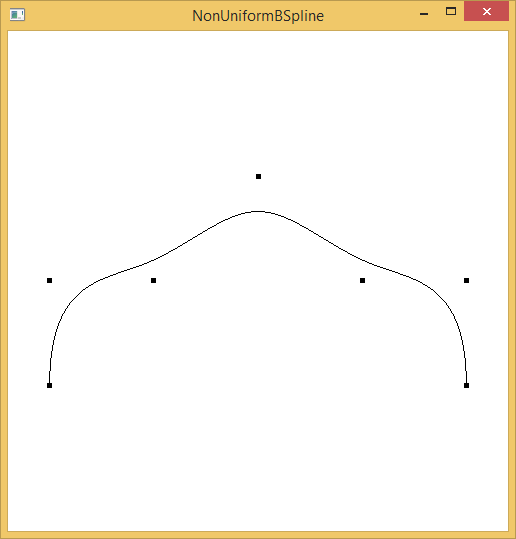
\includegraphics[width=8cm]{../Screenshots/ex-11/3-4.png}
\caption{Non-uniform B-Spline}
\label{fig:11-3-4}
\end{figure}

\subsection{Item 5}

I setup a NURBS curve with weights :\\

$ \{4, 3, 2, 1, 2, 3, 4\} $ \\

\noindent
The knot vector that is used in this item is\\


$ \{0, 0, 0, 0, 1, 1, 1, 2, 2, 2, 2\} $ \\

\noindent
A screenshot of the curve can be seen in Figure \ref{fig:11-3-5}.


\begin{figure}[hp]
\centering
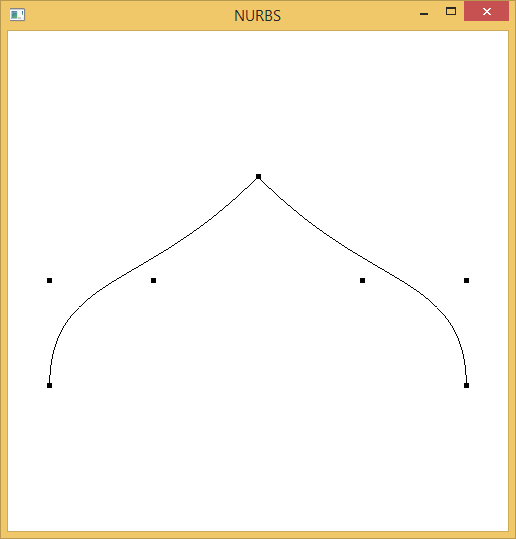
\includegraphics[width=8cm]{../Screenshots/ex-11/3-5.png}
\caption{NURBS (Non-Uniform Rational B-Spline)}
\label{fig:11-3-5}
\end{figure}


\section{Part 3}

I construct a set of control points. The set consists of 7x7, namely 49 control points. The edge control points with 7 units are non-linear. The edges has slight curvature. By setting 8 inner control points manually I create two hills. The resulting curve can be seen in Figure \ref{fig:11-4}

\begin{figure}[hp]
\centering
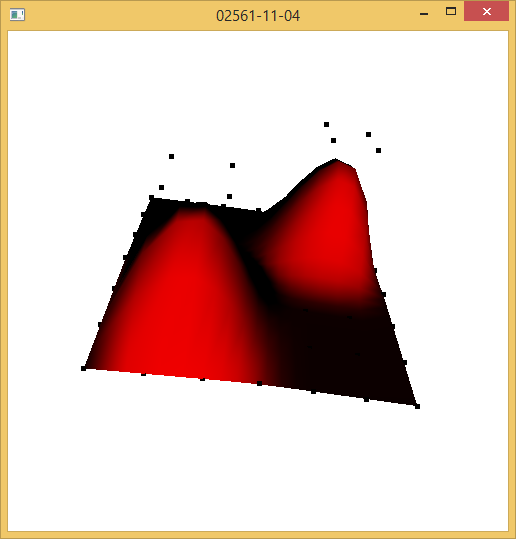
\includegraphics[width=8cm]{../Screenshots/ex-11/4.png}
\caption{NURBS surface}
\label{fig:11-4}
\end{figure}